\documentclass[10pt,conference]{IEEEtran}
\usepackage{cite}
\usepackage{amsmath,amssymb,amsfonts}
\usepackage{algorithmic}
\usepackage{graphicx}
\usepackage{textcomp}
\usepackage{xcolor}
\usepackage[hyphens]{url}
\usepackage{fancyhdr}
\usepackage{hyperref}
\hypersetup{hidelinks}
\usepackage{booktabs}
\usepackage{multirow}
\usepackage{array}
\usepackage{microtype}
\usepackage{balance}
\usepackage{tikz}
\usetikzlibrary{arrows.meta,positioning,fit,shapes.geometric}

\pdfpagewidth=8.5in
\pdfpageheight=11in
\newcommand{\hpcayear}{2027}
\newcommand{\draftvalue}[1]{\textcolor{red}{#1}}
\newcommand{\hpcasubmissionnumber}{4950}
\title{QuotientFlow: Learning Residual Flow Advantage for Symmetry-Reduced CGRA Mapping}
\newcommand{\hpcapubid}{0000--0000/00\$00.00}
\newcommand\hpcaauthors{Anonymous Authors}
\newcommand\hpcaaffiliation{Anonymous Affiliation}
\newcommand\hpcaemail{Anonymous Email}
\input{hpca-template}

\newcommand{\method}{\textsc{QuotientFlow}}
\newcommand{\scorer}{\textsc{FlowAdvantage}}
\newcommand{\mrrg}{MRRG}
\begin{abstract}
Mapping a dataflow graph (DFG) onto a coarse-grained reconfigurable array (CGRA) requires coupled placement and routing decisions under tight, time-expanded resource constraints. Existing heuristic mappers can make locally short routing choices that consume globally scarce resources, while exact formulations are too expensive to invoke at every search step. This paper presents \method, a deterministic beam mapper that derives state-conditioned guidance from a regularized fractional residual mapping problem. Routing- and compute-capacity duals provide a local first-order approximation to an action's opportunity cost; a two-tower graph neural network predicts the finite-action residual relative to an exact one-step child relaxation. The resulting \scorer{} ranks only legal native placement-and-route actions, and an optional top-$k$ mode applies exact child relaxations to a learned shortlist. A conservative quotient path is defined only for transforms that preserve the complete operation order and induce equivariant legal actions, scores, and successors. We integrate the method with Morpher and two independent legality paths. The current artifact validates integration with 148 regression tests and rejection of all eight deliberately corrupted native mappings. In a two-architecture \texttt{trmm} suffix-completion probe after a deterministic 40\% length prefix, proposal-only search matched the length baseline's route cost but required 3.3--4.0$\times$ longer; dual-linear and top-$4$ variants reached the fixed timeout. These results establish narrow functional correctness and expose relaxation cost. They do not establish end-to-end mapping quality, dual stability, learned-ranking quality, transfer, or quotient reduction.
\end{abstract}

\section{Introduction}
Coarse-grained reconfigurable arrays (CGRAs) combine spatially distributed functional units with a programmable interconnect, providing a flexible substrate for accelerating loop kernels. Their efficiency depends on the compiler's ability to map a dataflow graph (DFG) onto processing elements and route every dependence through a modulo-expanded interconnect. A poor placement can make later routes impossible even when each early choice appears locally inexpensive. Consequently, mapping remains a central obstacle to retargetable CGRA compilation~\cite{dresc,cgrame,modulo,himap}.

The difficulty is not merely the size of the search space. Placement and routing consume shared resources with highly nonuniform future value. A link on many remaining source-to-sink paths can be far more consequential than an equally long peripheral link. Local distance heuristics do not represent this opportunity cost. Negotiated-congestion routers such as PathFinder recover from overuse iteratively~\cite{pathfinder}, and simulated annealing can revise earlier placements, but both may spend substantial time discovering scarcity indirectly. Exact integer formulations expose global structure but scale poorly when solved repeatedly~\cite{cgrailp}. Learned mappers can amortize search, but handcrafted labels or end-to-end rewards provide only indirect supervision for the resource bottleneck that determines routability~\cite{lisa,rlmapping}.

Our key observation is that a partial mapping state defines a residual optimization problem whose routing-capacity dual variables approximate local marginal scarcity. Strong convexity makes the primal optimum unique, but it does not by itself make capacity multipliers unique under redundant constraints. We therefore treat the extracted shadow prices as a solver- and regularization-dependent first-order baseline whose stability must be measured. A discrete action can alter feasible endpoint assignments, path alternatives, and future cuts in ways that a parent-state linearization cannot capture, motivating a learned residual correction rather than an unconstrained policy.

\method{} combines two candidate reductions. First, \scorer{} ranks legal placement-and-route actions by adding a learned residual advantage to the parent relaxation's dual linearization; optional top-$k$ correction solves exact child relaxations only for the learned shortlist. Second, a conservative canonicalization can merge partial states only when an admitted transform is a symmetry of the complete ordered transition system. The first mechanism is intended to reduce child solves; the second is intended to remove duplicate state orbits. Neither changes the native candidate generator, but both require empirical validation before a quality or search-reduction claim is warranted.


\begin{figure}[t]
\centering
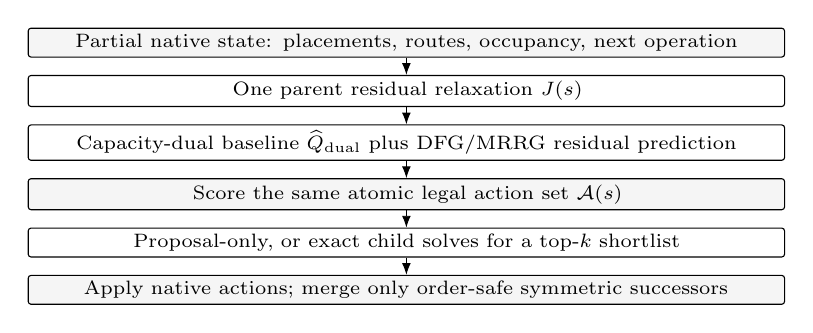
\begin{tikzpicture}[
  node distance=2.2mm,
  box/.style={draw, rounded corners=1pt, align=center, inner sep=2.1pt, text width=0.78\columnwidth, font=\scriptsize},
  arr/.style={-{Latex[length=1.5mm]}, line width=0.35pt}
]
\node[box,fill=black!4] (state) {Partial native state: placements, routes, occupancy, next operation};
\node[box,below=of state] (relax) {One parent residual relaxation $J(s)$};
\node[box,below=of relax] (score) {Capacity-dual baseline $\widehat Q_{\mathrm{dual}}$ plus DFG/MRRG residual prediction};
\node[box,below=of score,fill=black!4] (actions) {Score the same atomic legal action set $\mathcal A(s)$};
\node[box,below=of actions] (topk) {Proposal-only, or exact child solves for a top-$k$ shortlist};
\node[box,below=of topk,fill=black!4] (beam) {Apply native actions; merge only order-safe symmetric successors};
\draw[arr] (state)--(relax);
\draw[arr] (relax)--(score);
\draw[arr] (score)--(actions);
\draw[arr] (actions)--(topk);
\draw[arr] (topk)--(beam);
\end{tikzpicture}
\caption{\method{} scoring and search contract. Optimization and learning change scores, not the native legal-action universe. Canonicalization is admitted only when the full ordered transition contract is equivariant.}
\label{fig:overview}
\end{figure}


Figure~\ref{fig:overview} summarizes the scoring contract. We implement the method over Morpher's native DFG and modulo routing resource graph (MRRG) contracts~\cite{morpher}. The reference mapping is used only to identify a validated corpus; its placements, routes, occupancy, and score are not inputs. The available learned-method probe begins from an empty mapper state but delegates the first 40\% of operations to a deterministic length scorer. It is therefore a suffix-completion experiment, not end-to-end evidence for learned early decisions. Complete mappings are checked by both an independent serialized-contract validator and a native reimport path.

This paper makes four contributions:
\begin{itemize}
  \item A regularized fractional residual placement-and-routing formulation whose capacity multipliers define a testable first-order action baseline.
  \item \scorer, a residual-learning objective and two-tower GNN that predicts finite-action corrections while preserving the native legal-action universe.
  \item An order-safe state-orbit specification, deterministic beam search, and optional top-$k$ exact correction, with exactness claims explicitly conditioned on transition and score equivariance.
  \item A Morpher-native integration and evidence protocol that distinguishes legal mapping failure, timeout, and infrastructure error. The supplied evidence supports narrow correctness and runtime observations, not mapping-quality improvement.
\end{itemize}

\section{Background and Motivation}
\subsection{CGRA mapping}
A scheduled DFG is a directed graph $G_D=(V_D,E_D)$. Each operation $v\in V_D$ has an opcode and a legal modulo-time interval. For initiation interval (II) $I$, the architecture is expanded into an MRRG $G_R=(V_R,E_R)$ whose resources represent time-indexed datapaths, ports, switches, and links. A complete mapping assigns every operation to a compatible datapath and every dependence to a directed resource sequence satisfying temporal, occupancy, signal, memory-access, and recurrence constraints.

The mapper operates incrementally. A partial state $s$ contains operation placements $P_s$, routed dependences $R_s$, occupied compute resources $C_s$, and occupied routing resources $L_s$. A legal action $a$ places the next operation and atomically routes each newly closed dependence. Atomicity is important: evaluating a target placement without its required routes admits states that cannot occur in the native mapper.

The operation order is deterministic: ascending schedule level, descending fan-out, then stable node identifier. For a state $s$, the candidate generator enumerates compatible datapaths within the operation's schedule horizon, enumerates up to $k_p$ native routes per newly closed dependence, combines compatible route choices, and rejects actions that violate occupancy or signal compatibility. Search policies therefore compare scores over the same legal action set $\mathcal{A}(s)$.

\begin{table}[t]
\centering
\caption{Notation used throughout the paper. A bar denotes residual capacity after applying the native partial state.}
\label{tab:notation}
\begin{tabular}{ll}
\toprule
Symbol & Meaning \\
\midrule
$G_D=(V_D,E_D)$ & Scheduled dataflow graph \\
$G_R=(V_R,E_R)$ & II-expanded routing resource graph \\
$s$; $s_a$ & Partial native state; child after action $a$ \\
$\mathcal{A}(s)$ & Atomic legal actions exposed at $s$ \\
$J(s)$ & Optimal residual fractional objective \\
$\lambda_\ell,\mu_r$ & Routing- and compute-capacity duals \\
$Q^*(s,a)$ & Exact one-step relaxed action value \\
$A_{\mathrm{res}}(s,a)$ & Residual error of the dual estimate \\
$\kappa(s)$ & Exact canonical state key \\
\bottomrule
\end{tabular}
\end{table}

Three invariants constrain the design. \emph{Native legality} means that scoring never creates a placement or route outside the native candidate generator. \emph{Atomic action semantics} means that a placement is evaluated together with every dependence that becomes routable at that step. \emph{Score-only comparability} means that deterministic beam variants differ in scoring, not in candidate caps, route enumeration, operation order, or terminal checks. These invariants are required for attributing an outcome to guidance rather than to a different search universe.

\subsection{Why path length is insufficient}
A length-based policy minimizes the resources used by the current action. Let $c(a)$ be the sum of base costs for newly occupied routing resources plus any immediate placement cost. Two actions with the same $c(a)$ can have different consequences. One may consume a bridge in the residual graph, remove the only path between a remaining producer and consumer, or occupy a datapath needed by an unmatched opcode. These effects are state dependent and cannot be represented by a static edge weight.

A direct exact lookahead would apply each $a\in\mathcal{A}(s)$, solve the residual mapping problem for child state $s_a$, and rank by $c(a)+J(s_a)$, where $J$ is the relaxed residual objective. This is principled but expensive: a beam state may expose hundreds or thousands of native actions, and each child problem includes many flow variables. The design goal is therefore to approximate the ordering induced by exact child relaxation while solving at most one parent relaxation per state and a small number of child relaxations.

\subsection{Dual prices as local sensitivity}
For a convex residual problem, a capacity multiplier participates in a first-order sensitivity relation for marginal right-hand-side changes under standard regularity conditions~\cite{boyd}. A positive routing multiplier can therefore indicate that residual demand presses against that resource. However, the multiplier selected by a numerical solver need not be unique when constraints are redundant, and a native action removes a finite unit rather than an infinitesimal amount. We use the signal as an approximation derived from complete residual demand, not as a measured or solver-independent scarcity quantity.

Dual sensitivity is still a local approximation. Discrete actions remove whole units of capacity, change endpoint feasibility, and can alter the active set. The parent dual may thus rank many actions correctly while missing state transitions near cuts or compatibility boundaries. \method{} uses the dual estimate as a structured baseline and learns only the nonlinear residual.

\section{Residual Mapping Formulation}
\subsection{Variables and residual capacities}
Let $U_s=V_D\setminus\mathrm{dom}(P_s)$ be the unmapped operations and $D_s\subseteq E_D$ the unrouted dependences. For each $v\in U_s$ and compatible compute resource $r\in V_R$, $x_{v,r}\in[0,1]$ denotes fractional placement. For each residual dependence $e\in D_s$ and directed MRRG edge $\ell\in E_R$, $f_{e,\ell}\in[0,1]$ denotes fractional flow. Existing placements appear as fixed one-hot endpoint vectors. Existing routes and any optional knockout resource have zero residual capacity.

For residual dependence $e=(u,v)$ and routing node $q$, let $B_{q,\ell}$ be the directed incidence matrix, with $+1$ at the source and $-1$ at the destination of edge $\ell$. Let $\pi_v(q)$ denote either the fixed placement of an anchored operation or the fractional placement vector of an unmapped operation. The residual program is
\begin{align}
J(s)=\min_{x,f}\quad
&\sum_{e\in D_s}\sum_{\ell\in E_R} c_\ell f_{e,\ell}
 +\frac{\tau}{2}\sum_{v,r}x_{v,r}^2 \nonumber\\
&\hspace{10mm}+\frac{\tau}{2}\sum_{e,\ell}f_{e,\ell}^2 \label{eq:objective}\\
\text{s.t.}\quad
&\sum_{r\in\mathcal{C}(v)}x_{v,r}=1,
&&\forall v\in U_s, \label{eq:assign}\\
&\sum_{v\in U_s}x_{v,r}\leq \bar c_r(s),
&&\forall r, \label{eq:compute}\\
&\sum_{\ell\in E_R}B_{q,\ell}f_{e,\ell}
 =\pi_u(q)-\pi_v(q),
&&\substack{\forall e\in D_s,\\[-1pt]\forall q\in V_R}, \label{eq:flow}\\
&\sum_{e\in D_s} f_{e,\ell}\leq \bar b_\ell(s),
&&\forall \ell, \label{eq:capacity}\\
&0\leq x_{v,r}\leq1,\qquad 0\leq f_{e,\ell}\leq1. \nonumber
\end{align}
Here $\mathcal{C}(v)$ is the compatible compute-resource set, $\bar c_r(s)$ is residual compute capacity, and $\bar b_\ell(s)$ is residual routing capacity. The base cost $c_\ell$ distinguishes movement and register/wait resources. The quadratic term with $\tau>0$ makes the primal optimum unique. It is intended to reduce numerical variation, but it does not guarantee unique capacity multipliers; dual-ranking stability must therefore be established by a $\tau$/solver/tolerance sweep. The implementation uses CVXPY~\cite{cvxpy}, with a conic solver as primary and OSQP~\cite{osqp} as fallback.

Let $\lambda_\ell(s)\geq0$ be the dual of~\eqref{eq:capacity}, and $\mu_r(s)\geq0$ the dual of~\eqref{eq:compute}. The solver records assignment, flow, and capacity residuals; variable bounds; status; objective; solve time; and the fraction of positive duals. A state is scoreable only when the residual solve returns a permitted terminal status and passes numerical-health thresholds.

\subsection{Dual-linear action estimate}
A legal action $a$ occupies a target compute resource $r(a)$ and a set of previously free routing resources $L(a)$. Its parent-state dual estimate is
\begin{equation}
\widehat{Q}_{\mathrm{dual}}(s,a)=c(a)+\mu_{r(a)}(s)+\sum_{\ell\in L(a)}\lambda_\ell(s). \label{eq:dualbaseline}
\end{equation}
This is a first-order approximation of the objective increase caused by removing the action's resources from the parent residual problem. It is deterministic, permutation equivariant with respect to verified resource relabelings, and inexpensive once $J(s)$ has been solved.

Figure~\ref{fig:dualmotivation} illustrates why the baseline can distinguish equal-length routes while remaining only local. The oracle one-step value solves the exact relaxed child:
\begin{equation}
Q^*(s,a)=c(a)+J(s_a)-J(s), \label{eq:oracleq}
\end{equation}
where $s_a$ is the legal child state. We define the residual flow advantage
\begin{equation}
A_{\mathrm{res}}(s,a)=Q^*(s,a)-\widehat{Q}_{\mathrm{dual}}(s,a). \label{eq:advantage}
\end{equation}
The model predicts $A_{\mathrm{res}}$, not $Q^*$ directly. This decomposition supplies an interpretable baseline and permits dual-only and direct-$Q^*$ ablations. Whether it reduces target difficulty or improves held-out ranking is an empirical question, not a consequence of the definition.


\begin{figure}[t]
\centering
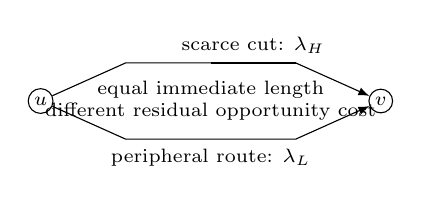
\begin{tikzpicture}[x=0.54cm,y=0.44cm,>=Latex,font=\scriptsize]
\node[draw,circle,inner sep=1.2pt] (s) at (0,1.5) {$u$};
\node[draw,circle,inner sep=1.2pt] (t) at (8,1.5) {$v$};
\coordinate (a1) at (2,2.6); \coordinate (a2) at (4,2.6); \coordinate (a3) at (6,2.6);
\coordinate (b1) at (2,0.4); \coordinate (b2) at (4,0.4); \coordinate (b3) at (6,0.4);
\draw[-{Latex[length=1.4mm]}] (s)--(a1)--(a2)--(a3)--(t);
\draw[-{Latex[length=1.4mm]}] (s)--(b1)--(b2)--(b3)--(t);
\draw[line width=1.0pt] (a2)--(a3);
\node[above] at (5,2.6) {scarce cut: $\lambda_H$};
\node[below] at (4,0.4) {peripheral route: $\lambda_L$};
\node[align=center] at (4,1.5) {equal immediate length\\different residual opportunity cost};
\end{tikzpicture}
\caption{Conceptual motivation for the dual baseline. Equal-length native routes can consume resources with different local capacity sensitivities. The finite child relaxation is still required to label errors caused by endpoint and active-set changes.}
\label{fig:dualmotivation}
\end{figure}


\section{The QuotientFlow Mapper}
\subsection{Graph representation and action features}
The model has separate towers for the DFG and MRRG. DFG node features encode operation type, normalized in/out degree, schedule phase, anchored status, and normalized anchored coordinates. The DFG tower performs five directed residual message-passing steps with separate incoming and outgoing aggregation. MRRG node features encode normalized space--time coordinates, degree, occupancy, boundary indicators, and a log-normalized compute dual. MRRG edge features encode resource kind, occupancy, residual availability, direction, and a log-normalized routing dual; the tower performs five directed edge-conditioned residual steps.

For action $a$, the head concatenates the next-operation and target-resource embeddings; mean and max pools of each graph; mean and max embeddings of newly occupied routing edges; and deterministic scalar features. The scalar features include immediate cost, occupied-resource fractions, alternative-path availability, bridge and edge-betweenness exposure, demand-to-cut ratios, parent objective and residual-health statistics, and the routing and compute terms of~\eqref{eq:dualbaseline}. Scalar features are standardized using the training split only.

\subsection{Labels and residual-learning objective}
Training groups are partial states with a common next operation and their complete bounded legal action set. For every retained action, label generation solves the exact child relaxation and computes~\eqref{eq:oracleq} and~\eqref{eq:advantage}. Let $m$ and $\sigma$ be the median and robust scale of training residuals. The clipped regression target is $y_a=\mathrm{clip}((A_{\mathrm{res}}(s,a)-m)/\sigma,-8,8)$. At inference,
\begin{equation}
\widehat{Q}_{\mathrm{FA}}(s,a)=\widehat{Q}_{\mathrm{dual}}(s,a)+\sigma g_\theta(s,a)+m. \label{eq:fascore}
\end{equation}
Lower values are preferred.

The groupwise training loss is
\begin{equation}
\mathcal{L}=\mathcal{L}_{\mathrm{list}}+\frac{1}{2}\mathcal{L}_{\mathrm{pair}}+\frac{1}{4}\mathcal{L}_{\mathrm{Huber}}, \label{eq:loss}
\end{equation}
where $\mathcal{L}_{\mathrm{list}}$ is cross entropy from a soft oracle distribution over exact action regrets, $\mathcal{L}_{\mathrm{pair}}$ is a regret-weighted logistic loss over materially separated pairs, and $\mathcal{L}_{\mathrm{Huber}}$ regresses $y_a$. Checkpoint selection is lexicographic: top-$4$ oracle recall, epsilon-optimal top-$1$, relative selected regret, and exact top-$1$. This criterion matches the intended use as a proposal mechanism rather than rewarding only global correlation.

\subsection{Optional Exact Top-\texorpdfstring{$k$}{k} Correction}
Proposal-only search ranks all legal actions by~\eqref{eq:fascore}. Top-$k$ search uses the same scores to select $k$ actions and replaces their scores with exact values from~\eqref{eq:oracleq}; all other actions receive infinite local score for that state. The comparison to full lookahead is valid only when both methods enumerate the same legal actions and differ solely in the number of child relaxations. Caches are keyed by architecture, DFG, partial-state, action, solver configuration, and source hashes to prevent cross-contract reuse.

\subsection{Deterministic beam search}
Figure~\ref{fig:algorithm} gives the complete search. Beam entries are ordered by cumulative score, action key, and stable state key. Successors with identical serialized native state are merged. A scorer may reject one state if its relaxation or feature contract is unavailable; other beam states continue. The mapper stops only on a complete legal mapping, no legal action, expansion limit, cancellation, or external timeout.

\begin{figure}[t]
\centering
\begin{minipage}{0.96\columnwidth}
\begin{algorithmic}[1]
\STATE \textbf{Input:} native problem $\mathcal{P}$, initial frontier $B_0$, scorer $S$, beam width $w$
\STATE $B\leftarrow B_0$
\FOR{operation $v$ in deterministic order}
  \STATE $C\leftarrow\emptyset$
  \FOR{each $(q,s)\in B$}
    \STATE $T\leftarrow$ compatible targets for $v$ in $s$
    \STATE $A\leftarrow$ atomic legal placement-route actions from $T$
    \STATE $z\leftarrow S(\mathcal{P},s,A)$
    \FOR{each finite-scored $(a,z_a)$}
      \STATE $s'\leftarrow\mathrm{Apply}(s,a)$
      \STATE insert or improve $C[\mathrm{Key}(s')]$ with $(q+z_a,s')$
    \ENDFOR
  \ENDFOR
  \IF{$C=\emptyset$} \STATE \textbf{return} valid mapping failure \ENDIF
  \STATE $B\leftarrow$ first $w$ entries of sorted $C$
\ENDFOR
\FOR{each complete state in sorted $B$}
  \IF{independent legality passes} \STATE \textbf{return} mapping \ENDIF
\ENDFOR
\STATE \textbf{return} legality failure
\end{algorithmic}
\end{minipage}
\caption{Deterministic native beam mapping. Candidate generation and legality are identical across scoring policies.}
\label{fig:algorithm}
\end{figure}

\subsection{Order-safe symmetry quotienting}
Let $v_1\prec\cdots\prec v_n$ be the complete deterministic operation order, including the stable-identifier tie break, and let $\rho(v_i)=i$. A DFG automorphism is admissible only if it preserves opcode, directed typed edges, schedule semantics, and the total rank $\rho$. Because $\rho$ is a total order, this condition may reduce the admissible DFG group to the identity. This restriction is deliberate: graph automorphism alone is insufficient when search transitions depend on a fixed ordered prefix.

For a state at depth $d$, an admissible joint transform $\gamma=(\gamma_D,\gamma_R)$ must also preserve the mapped prefix, architecture resource and edge classes, capacities, time phase, operation support, memory and recurrence semantics, and every native conflict relation used by action generation. In addition, it must satisfy the ordered transition contract
\begin{align}
\gamma\mathcal{A}(s)&=\mathcal{A}(\gamma s), \\
\gamma\,\mathrm{Apply}(s,a)&=\mathrm{Apply}(\gamma s,\gamma a), \\
z_s(a)&=z_{\gamma s}(\gamma a),
\end{align}
where the first equality denotes a bijection of legal atomic actions and $z$ is the active local scorer, including deterministic tie handling. A transform is not admitted merely because it is an automorphism of the unannotated DFG or MRRG.

For the admitted group $\Gamma(s)$, define $\mathrm{ser}(\gamma s)$ from the transformed ordered prefix, placements, compute occupancy, routing occupancy, routed-edge identifiers, and remaining operation sequence. The canonical key is
\begin{equation}
\kappa(s)=\min_{\gamma\in\Gamma(s)}\mathrm{ser}(\gamma s). \label{eq:canonical}
\end{equation}
Search retains the lowest cumulative-score representative per key. Under the three equivariance conditions above and invariant terminal legality and route cost, the orbit relation is a weighted bisimulation: exhaustive quotient and nonquotient searches have the same terminal orbits and best legal cost. For a finite beam, removing duplicate members of one orbit can expose additional non-equivalent states, so we claim a dominance reduction rather than identical heuristic output. No truncated group is called exact; if full verification or enumeration is unavailable, quotienting is disabled and ordinary byte-identical state merging remains enabled. Exhaustive small-instance action-bijection and terminal-set tests remain required before reporting quotient results.

\section{Native Morpher Integration}
\subsection{Contract extraction}
Morpher supplies a scheduled DFG, an II-expanded MRRG, and a native mapping schema~\cite{morpher}. The adapter imports operation keys, opcodes, basic-block mutex relations, datapath ownership, functional-unit support, operation latencies, resource conflicts, and directed MRRG connectivity. Missing latency or compatibility metadata fails closed. The mapper never synthesizes a default operation latency and never treats a structural JSON parse as evidence of functional legality.

A native state records operation placements, datapath occupancy, resource-to-signal occupancy, and routes keyed by DFG dependence. Native action generation reuses the architecture's route semantics, including broadcasts, mutex compatibility, mux conflicts, temporal deadlines, and memory-access restrictions. The final state exports through the same schema consumed by the independent validator and native reimport path.

\subsection{Reference isolation and suffix-probe initialization}
A reference mapping is hash-checked only to establish corpus provenance and native input consistency. It is forbidden as a source of placement, route, occupancy, score, or latency information during a paper run. The available probe initializes the mapper from an empty state, after which a deterministic length scorer maps
\begin{equation}
 d_0=\min\{|V_D|-1,\max(1,\lceil0.40|V_D|\rceil)\}
\end{equation}
operations. The complete beam frontier at depth $d_0$ is passed to the selected method, which controls only the suffix. Prefix time, expansions, actions, and routing attempts are reported separately. Because the learned method cannot revise the first $d_0$ decisions, this protocol is not used for a headline end-to-end claim. The frozen headline protocol sets $d_0=0$ for deterministic methods and reports 0\%, 20\%, and 40\% sensitivity only as a secondary analysis; conventional baselines start from their own empty native state under the same end-to-end wall budget.

\subsection{Legality and terminal status}
The independent checker operates only on serialized DFG, MRRG, and mapping documents. It verifies unique compute occupancy, directed route connectivity, opcode compatibility, schedule bounds, loop-carried timing, memory access, architecture identity, and II identity. A second path reconstructs a fresh native MRRG and imports the mapping. A result is a legal success only if the mapper reports completion and the required legality checks pass.

Terminal status is part of the scientific result. \textsc{ValidMappingFailure} means the mapper executed normally but exhausted its legal frontier. \textsc{Timeout} means an external wall bound terminated the process tree. \textsc{Error} denotes an invalid contract or infrastructure failure. Pending and running rows are nonresults. Aggregate quality comparisons must use identical paired sets of normally completed cells.

\section{Experimental Methodology}
\subsection{Questions}
The complete evaluation is organized around five questions:
\begin{enumerate}
  \item Do residual duals identify consequential routing resources?
  \item Does learned residual correction improve legal mapping success, minimum II, or route cost over length and dual-linear scoring?
  \item How much exact child-lookahead quality does top-$k$ retain, and at what runtime?
  \item Does exact quotienting reduce explored states without changing the best result?
  \item Does the method transfer across architecture topology, memory constraints, and array size?
\end{enumerate}
The supplied handoff contains narrow correctness evidence and a limited native probe, but not the paired or held-out data required to answer Questions 1--5. We report only the available results and define the evidence needed for each future claim.

\subsection{Workloads and architectures}
The frozen paper suite uses six established native kernels (\texttt{array\_add}, \texttt{array\_cond}, \texttt{gemm\_nt}, \texttt{fix\_fft}, \texttt{hpcg}, and \texttt{trmm}) and four compiler-derived kernels (\texttt{fir}, \texttt{conv2}, \texttt{conv3}, and \texttt{mac}). Kernel selection precedes observation of \method{} outcomes. The architecture set comprises A0, a standard $4\times4$ HyCUBE; A1, a standard $4\times4$ NoC; A2, a memory-constrained $4\times4$ HyCUBE; and A3, a held-out $8\times8$ HyCUBE~\cite{hycube}. A3 is excluded from training, checkpoint selection, and threshold selection.

\begin{table}[t]
\centering
\caption{Fixed mapping methods. All learned and deterministic beam methods use the same native candidate generator.}
\label{tab:methods}
\resizebox{\columnwidth}{!}{%
\begin{tabular}{ll}
\toprule
Method & Action score / search mechanism \\
\midrule
Length & Immediate native route length \\
Dual-linear & Eq.~\eqref{eq:dualbaseline} \\
Proposal & Learned score in Eq.~\eqref{eq:fascore} \\
Top-$k$ & Proposal shortlist, $k\in\{1,2,4,8\}$ exact child solves \\
Full lookahead & Exact child solve for every legal action \\
PathFinder & Native negotiated-congestion mapper \\
Simulated annealing & Native mapper, seeds 11, 23, and 37 \\
\bottomrule
\end{tabular}}
\end{table}

\subsection{Metrics and pairing}
For each kernel, architecture, seed, and budget cell, the artifact records status, legality, success, II attempts, minimum mapped II, route cost, mapped operations, expansions, generated actions, routing attempts, parent and child solves, cache hits, peak memory, and stage times. Quality deltas are computed only on identical paired terminal cells. The planned aggregate uses 10,000 paired bootstrap resamples with fixed seed 24072026 and reports the estimate, 95\% interval, paired count, and per-kernel/per-architecture values. An interval including zero is not described as statistically reliable.

\subsection{Evidence provenance and reproducibility}
Each run is an isolated process with an immutable manifest, heartbeat, external process-tree timeout, schema-validated temporary result, file-system synchronization, and atomic rename. The record binds source, configuration, checkpoint, kernel, architecture, solver, and native-input hashes. Cache keys include the partial state and solver contract, preventing reuse across semantically different problems. The architecture and kernel census is frozen before reading learned-method outcomes; A3 remains excluded from model and threshold selection.

The evaluation treats operational state as data. A legal-success row requires method completion and the configured legality checks. A normal search exhaustion is a valid mapping failure. Timeout, error, unsupported, running, and pending remain distinct statuses and are never inserted into a success denominator without an explicitly named success-under-budget metric. This distinction is essential when solver overhead differs sharply between methods.

\subsection{Learning and dual-validation disclosures}
Any quality-bearing learned result must report the split unit and complete train/validation/test membership; counts of state groups and actions; trajectory-level leakage prevention; model dimensions and parameter count; optimizer, learning-rate schedule, batch construction, epochs, seeds, checkpoint rule, and training cost; and exact-child label success, rejection, and fallback rates. Held-out reporting must include top-$1$ and top-$k$ oracle recall, selected regret, and rank correlation for dual-only, scalar-only, GNN-only, no-dual, direct-$Q^*$, and residual-target variants. The current handoff does not contain these values, so the paper does not claim reproducible learned ranking.

Dual validation is separate from model validation. On held-out states, the frozen analysis compares each positive multiplier with a finite resource-knockout difference, evaluates action-regret rank correlation and top-$k$ recall, sweeps $\tau$, solver, and tolerances, and reports positive-dual, fallback, rejected-state, and solver-disagreement rates. Categorical wording such as ``quantifies scarcity'' is not used unless these measurements support it.

\begin{table}[t]
\centering
\caption{Evidence available at artifact freeze and its admissible interpretation.}
\label{tab:claims}
\begin{tabular}{>{\raggedright\arraybackslash}p{0.29\columnwidth}>{\raggedright\arraybackslash}p{0.58\columnwidth}}
\toprule
Evidence & Supports \\
\midrule
Regression and adversarial legality tests & Native-state and checker correctness \\
Two-architecture terminal proposal probe & Executability, legality, and measured overhead \\
Incomplete length snapshot & Protocol coverage; no paired method delta \\
Top-$4$ timeout rows & Runtime boundary; no mapping failure \\
Missing paired core matrix & No success, II, route-cost, or portability claim \\
\bottomrule
\end{tabular}
\end{table}

\section{Results}
\subsection{Functional correctness}
Table~\ref{tab:correctness} summarizes the evidence available in the handoff. The repository's regression suite reports 148 passing tests with plugin autoload disabled to avoid an unrelated environment dependency. These tests cover architecture and DFG construction, flow conservation, relaxation health, equivariance, native mapper state transitions, proposal compatibility, caching, seeded simulated annealing, manifest construction, memory layout, and queue semantics.

The stronger negative test begins from a legal native \texttt{gemm\_nt} mapping and independently introduces eight faults. They cover duplicate compute occupancy, disconnected direction, incompatible multiplication placement, schedule-window violation, recurrence overrun, illegal memory placement, wrong architecture hash, and wrong II. Both the serialized-contract checker and the native reimport validator reject all eight through structured validation paths; crashes and timeouts are not credited as rejection.

\begin{table}[t]
\centering
\caption{Available correctness evidence. ``Native'' denotes a fresh native reconstruction/reimport check.}
\label{tab:correctness}
\begin{tabular}{lrr}
\toprule
Check & Passed & Total \\
\midrule
Regression tests & 148 & 148 \\
Independent negative legality & 8 & 8 \\
Native negative legality & 8 & 8 \\
Deterministic prefix repeatability & 2 & 2 \\
Atomic native PathFinder smoke & 1 & 1 \\
\bottomrule
\end{tabular}
\end{table}

\subsection{Baseline coverage}
The extended length-baseline snapshot contains 13 immutable rows. Eight are normally terminal: three legal successes and five valid mapping failures. One row timed out, one reported a contract error, two were still running, and one was pending at artifact freeze. Table~\ref{tab:lengthstatus} reports the rows without imputing outcomes. The three successful \texttt{trmm} cells map all 11 operations at II 4 with route costs 71, 72, and 71 on A0, A1, and A2, respectively. The valid mapping failures stop at 15/20 operations for \texttt{array\_add} A0, 20/25 and 16/25 for \texttt{array\_cond} A1/A2, and 12/24 and 15/24 for \texttt{hpcg} A0/A1.

\begin{table}[t]
\centering
\caption{Length-baseline snapshot. Nonterminal and abnormal rows are coverage information, not quality outcomes.}
\label{tab:lengthstatus}
\begin{tabular}{lr}
\toprule
Status & Rows \\
\midrule
Legal success (\textsc{Done}) & 3 \\
\textsc{ValidMappingFailure} & 5 \\
\textsc{Timeout} & 1 \\
\textsc{Error} & 1 \\
Running & 2 \\
Pending & 1 \\
\midrule
Total & 13 \\
\bottomrule
\end{tabular}
\end{table}

This snapshot is insufficient for a comparative claim because the learned and conventional baselines do not share the same complete paired terminal set. It documents native baseline coverage and the cost of exact route enumeration, particularly on A3; it does not validate the 40\% suffix protocol as an end-to-end comparison.

\subsection{Strict native FlowAdvantage probe}
Table~\ref{tab:probe} presents the only complete cross-method probe in the supplied artifact. It uses \texttt{trmm} on A0 and A2, a deterministic 40\% length prefix, beam width 4, action limit 24, at most 5000 expansions, and a 600-s external wall bound. Length and proposal-only search complete legal mappings on both architectures with identical route cost 71. Proposal-only performs 22 parent relaxations and no child solves. Its wall time is 468.48~s on A0 and 481.49~s on A2, compared with 117.44~s and 146.61~s for length, corresponding to 3.99$\times$ and 3.28$\times$ overhead.

Dual-linear reaches six of eleven operations after four parent solves on each architecture and times out. Top-$4$ reaches five operations and times out before a complete result. A timeout is not evidence of mapping failure, so neither method contributes a route-cost or success comparison. The probe demonstrates that model-guided native scoring is executable and legal, while repeated parent/child relaxation dominates the present implementation.

\begin{table*}[t]
\centering
\caption{Strict native \texttt{trmm} probe. A dash denotes no complete mapping; timeout rows are excluded from quality comparisons.}
\label{tab:probe}
\begin{tabular}{llrrrrrr}
\toprule
Architecture & Method & Status & Mapped ops & Route cost & Parent solves & Child solves & Wall time (s) \\
\midrule
A0 $4\times4$ HyCUBE & Length & Done & 11/11 & 71 & 0 & 0 & 117.44 \\
A0 $4\times4$ HyCUBE & Dual-linear & Timeout & 6/11 & -- & 4 & 0 & 601.33 \\
A0 $4\times4$ HyCUBE & Proposal & Done & 11/11 & 71 & 22 & 0 & 468.48 \\
A0 $4\times4$ HyCUBE & Top-$4$ & Timeout & 5/11 & -- & 0 & -- & 602.12 \\
\midrule
A2 memory-constrained HyCUBE & Length & Done & 11/11 & 71 & 0 & 0 & 146.61 \\
A2 memory-constrained HyCUBE & Dual-linear & Timeout & 6/11 & -- & 4 & 0 & 602.22 \\
A2 memory-constrained HyCUBE & Proposal & Done & 11/11 & 71 & 22 & 0 & 481.49 \\
A2 memory-constrained HyCUBE & Top-$4$ & Timeout & 5/11 & -- & 0 & -- & 602.00 \\
\bottomrule
\end{tabular}
\end{table*}

\subsection{What the current results establish}
The evidence supports three conclusions. First, the native adapter and state transitions are testable under both positive and adversarial legality checks. Second, the proposal scorer can complete a native mapping without consuming the reference witness and without changing the legal action universe. Third, relaxation cost is currently too high for the intended top-$k$ hierarchy under a 600-s cell budget. The evidence does \emph{not} establish improved mapping success, II, route cost, portability, or quotient-search reduction. Those claims require the paired matrix and ablations described in Section~VI.

\section{Discussion}
\subsection{What remains to validate about the first-order baseline}
The probe establishes neither usefulness nor stability of the dual decomposition. It does identify an implementation constraint: solving the native residual program at each beam state must be amortized or compiled more aggressively. The parent multiplier score is attractive because it is derived from complete residual demand, yields a transparent dual-linear ablation, and can be compared directly with finite-resource knockout differences. Those properties motivate the hypothesis; they do not demonstrate that the baseline outperforms length or remains invariant across solver settings. A competitive implementation should reuse compiled problem structure, warm-start solver state, batch feature/model evaluation, and invoke child solves only after the proposal shortlist is stable.

\subsection{Claim requirements for the complete evaluation}
The headline comparison must pair PathFinder, three seeded simulated-annealing runs, length, dual-linear, proposal, and top-$4$ on identical kernel/architecture/II/budget cells. Full lookahead should be restricted to a frozen balanced subset because of cost. The parent ablation must use a genuinely no-parent checkpoint; a model trained or evaluated with parent dual features cannot be relabeled as no-parent. Exact quotienting must be evaluated with exhaustive equivalence checks on small cases and expansion reduction on larger cases. A3 remains held out until all models and thresholds are frozen.

\subsection{Cost structure and implementation priorities}
The method's cost follows directly from the decision hierarchy. For a partial state, the residual program has placement variables proportional to the number of unmapped-operation/compatible-resource pairs and flow variables proportional to $|D_s||E_R|$. A proposal step requires one parent solve, graph and scalar feature construction, one batched GNN evaluation over the legal action group, and ordinary beam insertion. Top-$k$ correction adds $k$ child solves for each scored state; full lookahead adds $|\mathcal{A}(s)|$ child solves. Thus, the learned proposal is useful only when model and feature cost are small relative to the child solves it removes. The strict probe confirms that the present dominant term is the relaxation path, not neural inference, but the supplied timing does not isolate solver setup from numerical iterations.

Several optimizations preserve the method's semantics. The sparse constraint matrices for a fixed DFG--MRRG pair can be compiled once, with partial-state occupancy, endpoint anchors, and optional knockout resources applied through parameters. Parent and child problems differ primarily in right-hand sides and residual capacities, making warm starts and factorization reuse natural. Action scoring can batch all targets and route choices for a state; graph embeddings can be reused across the action group; and state-independent architecture statistics can be cached by the architecture hash. These changes reduce repeated work without changing labels, the legal action universe, or the exact top-$k$ definition.

The symmetry path has a different tradeoff. Canonicalization costs are proportional to the number of accepted joint transforms times the serialized state size. This overhead is justified only when it eliminates enough beam duplicates or relaxation solves. The implementation therefore needs per-instance accounting of accepted automorphisms, canonicalization time, merge count, expansions avoided, and downstream solves avoided. An exactness-preserving skip is preferable to a large group traversal that cannot amortize its own cost.

Finally, numerical diagnostics must remain visible. Near-zero or unstable duals can make the linear baseline uninformative even when the primal relaxation is feasible; an infeasible or unhealthy child solve cannot be converted into a finite oracle label. The artifact records solver status and residual checks so these cases can be separated from search failure. A complete evaluation should report the frequency of scoreable parent states, rejected labels, fallback solves, and cache hits alongside mapping outcomes.

\subsection{Threats to validity and limitations}
\emph{Construct validity.} The fractional formulation relaxes discrete signal conflicts and path choices; $J(s)$ is guidance, not a legality certificate. Route cost is also only one mapping-quality dimension, so the complete study must report success, minimum II, routing failures, and compiler time.

\emph{Internal validity.} Solver tolerances, multiplier nonuniqueness, cache reuse, candidate truncation, prefix depth, and stochastic baselines can confound a score comparison. The protocol therefore records residual health, hashes cache contracts, holds the action universe fixed across deterministic variants, uses zero-prefix headline comparisons, and reports multiple simulated-annealing seeds with uncertainty. Reference mappings are isolated from search to avoid witness leakage.

\emph{External validity.} The learned correction depends on the representativeness of sampled partial states, actions, kernels, and architectures. The frozen A3 holdout and compiler-derived kernels test only a limited form of transfer; conclusions should not be generalized to arbitrary CGRA organizations without additional native contracts.

\emph{Symmetry and current evidence.} DFG graph automorphisms that do not preserve the complete total operation order are excluded, even if this leaves only the identity. Architecture transforms are admitted only under the ordered transition and score-equivariance contract. Exact groups may still be too large to enumerate, in which case the method reports a skip. The current artifact contains no completed quotient-versus-nonquotient terminal-set experiment and no evidence that relaxation guidance improves mapping quality.

\section{Related Work}
\textbf{CGRA mapping.} DRESC established retargetable modulo mapping with architecture-aware placement and routing~\cite{dresc}. CGRA-ME provides architecture modeling and both heuristic and optimization-based mapping infrastructure~\cite{cgrame,cgrailp}. Modulo graph embedding and hierarchical abstraction improve quality or scalability through structured search~\cite{modulo,himap}. Morpher integrates architecture description, compilation, simulation, and generation~\cite{morpher}. Rewire instead coordinates placement and routing for multiple DFG nodes by sharing routing information during candidate construction~\cite{rewire}. A common-contract comparison remains necessary because that multi-node search space and termination policy differ from the atomic beam interface used here.

\textbf{Learned mapping guidance.} Deep reinforcement learning has been used for CGRA DFG mapping~\cite{rlmapping}; Zhuang et al. combine a GNN representation with reinforcement learning and routing exploration~\cite{zhuanggnn}; and LISA learns portable DFG labels that guide simulated annealing~\cite{lisa}. These works make GNN use, routing awareness, and learned CGRA guidance prior art. The narrower proposed distinction is the action-level decomposition into a residual-relaxation capacity baseline, a learned finite-action correction labeled by exact child relaxations, and optional exact top-$k$ reevaluation under an unchanged native atomic-action contract. The current results do not establish superiority over these systems.

\textbf{Learning expensive search decisions.} Gasse et al. train a GNN to imitate strong branching, replacing repeated expensive child-relaxation evaluations with a learned branching policy~\cite{gasse}. The methodological analogy is direct: both learn from a costly relaxation-based expert and must evaluate prediction quality jointly with policy overhead. \method{} differs in the CGRA-native placement-route action contract, the explicit parent-dual residual target, and optional exact top-$k$ correction rather than pure imitation.

\textbf{Congestion, duals, and symmetry.} PathFinder updates congestion costs through negotiated routing~\cite{pathfinder}, while convex duality provides local marginal sensitivity under regularity assumptions~\cite{boyd}. Symmetry reduction in integer and constraint programming relies on preserving the actual search problem, not merely an unannotated graph automorphism~\cite{margot,gentsym}. Accordingly, \method{} restricts quotienting to the complete ordered transition system and treats exhaustive action-bijection and terminal-set tests as mandatory evidence.

\section{Conclusion}
This paper specified \method, a deterministic CGRA mapping framework that combines a residual-relaxation capacity baseline, learned action-level correction, optional exact top-$k$ lookahead, and order-safe state-orbit reduction. The formulation separates local optimization sensitivity from the finite effect of a native atomic action, while the Morpher integration preserves a common legal action universe, isolates reference mappings from search, and distinguishes mapping failure from operational failure. The supplied evidence supports narrow integration correctness and a two-architecture suffix probe; it also shows that repeated relaxation is currently too expensive. Acceptance-level claims require zero-prefix paired end-to-end results, learned-ranking and dual-stability measurements, conventional and closest learned baselines, exhaustive quotient equivalence tests, held-out transfer, and quality-versus-time analysis.

\clearpage
\balance
\begin{thebibliography}{99}
\bibitem{dresc}
B. Mei, S. Vernalde, D. Verkest, H. De Man, and R. Lauwereins, ``DRESC: A retargetable compiler for coarse-grained reconfigurable architectures,'' in \emph{Proc. IEEE Int. Conf. Field-Programmable Technology (FPT)}, 2002, pp. 166--173.

\bibitem{cgrame}
S. A. Chin, N. Sakamoto, A. Rui, J. Zhao, J. H. Kim, Y. Hara-Azumi, and J. H. Anderson, ``CGRA-ME: A unified framework for CGRA modelling and exploration,'' in \emph{Proc. IEEE Int. Conf. Application-Specific Systems, Architectures and Processors (ASAP)}, 2017, pp. 184--189.

\bibitem{modulo}
H. Park, K. Fan, M. Kudlur, and S. Mahlke, ``Modulo graph embedding: Mapping applications onto coarse-grained reconfigurable architectures,'' in \emph{Proc. Int. Conf. Compilers, Architecture and Synthesis for Embedded Systems (CASES)}, 2006, pp. 136--146.

\bibitem{himap}
D. Wijerathne, Z. Li, A. Pathania, T. Mitra, and L. Thiele, ``HiMap: Fast and scalable high-quality mapping on CGRA via hierarchical abstraction,'' in \emph{Proc. Design, Automation and Test in Europe Conf. (DATE)}, 2021, pp. 1192--1197.

\bibitem{pathfinder}
L. McMurchie and C. Ebeling, ``PathFinder: A negotiation-based performance-driven router for FPGAs,'' in \emph{Proc. ACM Int. Symp. Field-Programmable Gate Arrays (FPGA)}, 1995, pp. 111--117.

\bibitem{hycube}
M. Karunaratne, A. Kulkarni Mohite, T. Mitra, and L.-S. Peh, ``HyCUBE: A CGRA with reconfigurable single-cycle multi-hop interconnect,'' in \emph{Proc. ACM/IEEE Design Automation Conf. (DAC)}, 2017, pp. 45:1--45:6, doi: 10.1145/3061639.3062262.

\bibitem{cgrailp}
S. A. Chin and J. H. Anderson, ``An architecture-agnostic integer linear programming approach to CGRA mapping,'' in \emph{Proc. ACM/ESDA/IEEE Design Automation Conf. (DAC)}, 2018, pp. 1--6.

\bibitem{lisa}
Z. Li, D. Wu, D. Wijerathne, and T. Mitra, ``LISA: Graph neural network based portable mapping on spatial accelerators,'' in \emph{Proc. IEEE Int. Symp. High-Performance Computer Architecture (HPCA)}, 2022, pp. 444--459.

\bibitem{rlmapping}
D. Liu, S. Yin, G. Luo, J. Shang, L. Liu, S. Wei, Y. Feng, and S. Zhou, ``Data-flow graph mapping optimization for CGRA with deep reinforcement learning,'' \emph{IEEE Trans. Computer-Aided Design of Integrated Circuits and Systems}, vol. 38, no. 12, pp. 2271--2283, 2019.

\bibitem{morpher}
D. Wijerathne, Z. Li, and T. Mitra, ``Accelerating edge AI with Morpher: An integrated design, compilation and simulation framework for CGRAs,'' arXiv:2309.06127, 2023.

\bibitem{boyd}
S. Boyd and L. Vandenberghe, \emph{Convex Optimization}. Cambridge, U.K.: Cambridge Univ. Press, 2004.

\bibitem{cvxpy}
S. Diamond and S. Boyd, ``CVXPY: A Python-embedded modeling language for convex optimization,'' \emph{J. Machine Learning Research}, vol. 17, no. 83, pp. 1--5, 2016.

\bibitem{osqp}
B. Stellato, G. Banjac, P. Goulart, A. Bemporad, and S. Boyd, ``OSQP: An operator splitting solver for quadratic programs,'' \emph{Mathematical Programming Computation}, vol. 12, pp. 637--672, 2020.

\bibitem{graphsage}
W. L. Hamilton, R. Ying, and J. Leskovec, ``Inductive representation learning on large graphs,'' in \emph{Advances in Neural Information Processing Systems}, 2017, pp. 1025--1035.

\bibitem{zhuanggnn}
Y. Zhuang, Z. Zhang, and D. Liu, ``Towards high-quality CGRA mapping with graph neural networks and reinforcement learning,'' in \emph{Proc. IEEE/ACM Int. Conf. Computer-Aided Design (ICCAD)}, 2022, pp. 61:1--61:9, doi: 10.1145/3508352.3549458.

\bibitem{rewire}
Z. Li, D. Wu, D. Wijerathne, D. Chen, H. Li, C. Tan, and T. Mitra, ``Rewire: Advancing CGRA mapping through a consolidated routing paradigm,'' in \emph{Proc. ACM/IEEE Design Automation Conf. (DAC)}, 2025, pp. 1--7, doi: 10.1109/DAC63849.2025.11133240.

\bibitem{gasse}
M. Gasse, D. Ch\'{e}telat, N. Ferroni, L. Charlin, and A. Lodi, ``Exact combinatorial optimization with graph convolutional neural networks,'' in \emph{Advances in Neural Information Processing Systems}, vol. 32, 2019, pp. 15554--15566.

\bibitem{margot}
F. Margot, ``Symmetry in integer linear programming,'' in \emph{50 Years of Integer Programming 1958--2008}, M. J\"unger, T. M. Liebling, D. Naddef, G. L. Nemhauser, W. R. Pulleyblank, G. Reinelt, G. Rinaldi, and L. A. Wolsey, Eds. Berlin, Germany: Springer, 2010, pp. 647--686.

\bibitem{gentsym}
I. P. Gent, K. E. Petrie, and J.-F. Puget, ``Symmetry in constraint programming,'' in \emph{Handbook of Constraint Programming}, F. Rossi, P. van Beek, and T. Walsh, Eds. Amsterdam, The Netherlands: Elsevier, 2006, pp. 329--376.
\end{thebibliography}

\appendices
\section{AI Use}
OpenAI ChatGPT was used for editorial restructuring, LaTeX assistance, and generation of the two conceptual schematic figures in this revision. It was not used to generate experimental measurements. The authors remain responsible for verifying all technical claims, equations, citations, source changes, and reported results before submission.

\end{document}
